Computational Aeroacoustics is unique in that solvers are required to be nondissipative, nondispersive, and isotropic in nature. This presents differences when considering discretisation compared to traditional CFD solvers, which often contain spatial discretisation schemes that are dispersive, anisotropic, and sometimes highly dissipative - all by choice to artificially control and damp the solutions.

When considering the propagation of a simple wave, a number of true analytical solutions exist - such as Burgers' equation \cite{landajuela2011burgers}. However, these solutions are limited in that they cannot be applied to propagation of a wave governed by alternative equations - such as the Euler equations used here. Numerical methods are used instead to provide accurate approximations for the partial differential equations (PDEs), where exact solutions are unknown or too complicated to determine in a closed form \cite{suli2003numanalys}. The described Euler equations (Section \ref{GovEqSection}) contain both spatial and temporal derivatives, and so require discretisation via approximations for both. The following outlines the methods used to write a linear Euler CAA solver in MATLAB, with additional augmented PML equations.

\subsubsection{Spatial Discretisation}

A first order derivative at the $i$th node can be approximated using a finite difference method (FDM) which considers the values of the cells around it - using what is termed as a stencil. The general form of FDM with uniform grid and stencil $i = \cdots -2, -1, 0, 1, 2 \cdots$ folllows as


\begin{equation}\label{FDMEquation}
    \left( \frac{\partial \mathbf{U}}{\partial x} \right)_{i} \approx
    \frac{\cdots + a_{-2} \mathbf{U}_{i-2} + a_{-1} \mathbf{U}_{i-1} + a_0 \mathbf{U}_{i} + a_1 \mathbf{U}_{i+1} + a_2 \mathbf{U}_{i+2} + \cdots}{\Delta x}
    = \frac{1}{\Delta x} \sum^M_{j=-N} a_j \mathbf{U}_{i+j}
\end{equation}



where there are $M$ values to the right and $N$ values to the left of the $i$th node, with weights $a_i$. If $M=N$, the scheme is said to be central difference. If one is greater than the other, then the scheme is forwards or backwards in its sampling of surrounding cells.

The weights are typically determined in a standard scheme by expanding the RHS of Equation \ref{FDMEquation} using a Taylor series of $\Delta x$, and then equating the coefficients using the same powers. This method yields weights which provide consistent, stable, and converged solutions, but does not guarantee accurate wave solutions for small amplitudes waves (when comparing the resolved characteristics with those of the governing Euler equations) \cite{spisso2007overviewfd}.

\textcite{hardin1995caaworkshop} conclude that in order to achieve this accuracy for small amplitude waves, high-order optimised schemes with a wide capacity for resolving wavenumbers are necessary. As was discussed in Section \ref{DispRelaStabSection}, wave propagation characteristics are determined by the dispersion relations. To assess a scheme's potential for wavenumber resolution, the scheme is applied to a similar ansatz of $e^{-ikx}$ \footnote[1]{the $e^{\mathrm{i}\omega t}$ term in Equation \ref{eq:OGAnsatz} refers to periodic waveforms, not transient, and can be omitted for brevity due to its appearance in all terms} to get the approximated derivative. First, consider the exact solution of the derivative
\begin{equation}
    \frac{\mathrm{d}e^{-\mathrm{i}kx}}{\mathrm{d}x} = -\mathrm{i}k e^{-\mathrm{i}kx}
\end{equation}
Then using the general form from Equation \ref{FDMEquation} the approximation is found as
\begin{equation}
    \frac{\mathrm{d}e^{-\mathrm{i}kx}}{\mathrm{d}x} \approx \frac{1}{\Delta x} \sum^M_{j=-N} a_j e^{-\mathrm{i}k\left(x+j\Delta x\right)} \\
    = - \mathrm{i}\Tilde{k}e^{-\mathrm{i}kx}
\end{equation}
where
\begin{equation}
    \Tilde{k} = \frac{\mathrm{i}}{\Delta x} \sum^M_{j=-N} a_j e^{-\mathrm{i}kj\Delta x}
\end{equation}

This allows for comparison between the exact wavenumber $k\Delta x$, and the modified (approximated) wavenumber $\Tilde{k} \Delta x$ using stencils of coefficients. The schemes currently used in CAA vary in implementation and derivation of the stencils. For this project, a small number of schemes are contrasted and compared. The first is the dispersion-relation preserving scheme (DRP) created by \textcite{tam193DRP}. Briefly summarised, if both systems of equations (7-point high-order FD scheme and Euler equations) have the same dispersion relations, then the numerical solutions of the FD scheme will have the same wave propagation characteristics (nondissipative, nondispersive), wave modes (acoustic, vorticity, entropy), and wave speeds at the governing Euler equations. Conclusively, optimising the FD scheme for dispersion relations bolsters the accuracy for CAA solutions - hence the dispersion-relation preserving name. The DRP scheme forms a self-contained time marching scheme, rather than segregating out the spatial and temporal discretisations. Alternatively, \textcite{zingg1996HighAccFD} present a 7-point optimised FD scheme which is paired with an explicit six-stage time-marching Runge-Kutta scheme. This scheme is optimised slightly differently, where the stencil is found through Fourier analysis and by minimising the max phase and amplitude errors for waves resolved by more than 10 points per wavelength (PPW). The result is a scheme capable of simulating long-distance wave radiation, which has many useful applications. Lastly a selection of standard 7, 5, and 3 point stencils are compared, which simply use Taylor expansion and equating of coefficients. Figure \ref{fig:FD} demonstrates the ability of the stencils to resolve waves over a range of wavenumbers, and shows that of the compared stencils - the DRP \cite{tam193DRP} scheme is the most promising for resolving higher wavenumbers (short wave components).


\begin{figure}[h!]
\centering
\makebox[0pt]{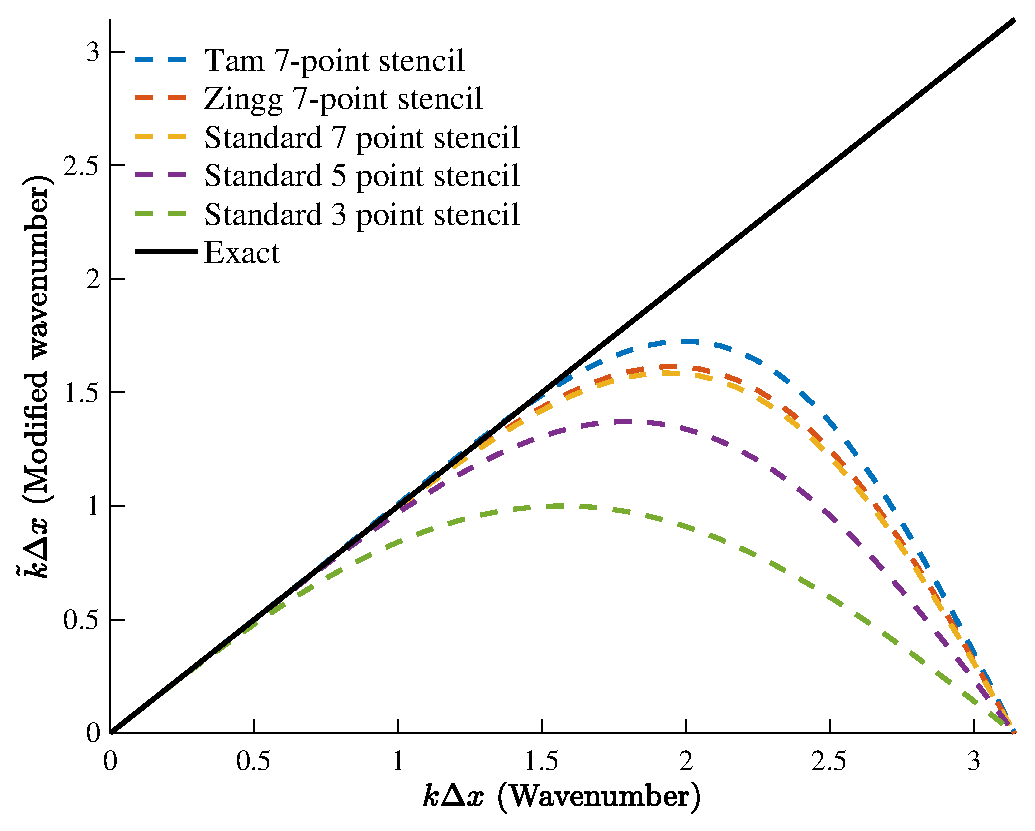
\includegraphics[width=8cm]{Figures/TechnicalAchievement/NumMeth/WavenumberPlot.eps}}
\caption{Comparison of various standard and optimised finite difference schemes from \textcite{tam193DRP} and \textcite{zingg1996HighAccFD}, showing wavenumber (exact) vs modified wavenumber (approximation by FD scheme).}
\label{fig:FD}
\end{figure}


Schemes do exist which are able to resolve higher wavenumbers (shorter components), such as \textcite{lele1992cfd}, but these use tridiagonal and pentadiagonal matrices (band matrices) which must be inverted - trading exceptional performance (spectral method-like resolution \cite{zhu2007caahofds}) for near massive computational effort. 